\hypertarget{stm32f4xx__hal__exti_8c}{}\section{Dokumentacja pliku S\+T\+M/\+W\+D\+S\+\_\+\+Kosc\+\_\+\+Linux/\+Drivers/\+S\+T\+M32\+F4xx\+\_\+\+H\+A\+L\+\_\+\+Driver/\+Src/stm32f4xx\+\_\+hal\+\_\+exti.c}
\label{stm32f4xx__hal__exti_8c}\index{S\+T\+M/\+W\+D\+S\+\_\+\+Kosc\+\_\+\+Linux/\+Drivers/\+S\+T\+M32\+F4xx\+\_\+\+H\+A\+L\+\_\+\+Driver/\+Src/stm32f4xx\+\_\+hal\+\_\+exti.\+c@{S\+T\+M/\+W\+D\+S\+\_\+\+Kosc\+\_\+\+Linux/\+Drivers/\+S\+T\+M32\+F4xx\+\_\+\+H\+A\+L\+\_\+\+Driver/\+Src/stm32f4xx\+\_\+hal\+\_\+exti.\+c}}


E\+X\+TI H\+AL module driver. This file provides firmware functions to manage the following functionalities of the Extended Interrupts and events controller (E\+X\+TI) peripheral\+:  


{\ttfamily \#include \char`\"{}stm32f4xx\+\_\+hal.\+h\char`\"{}}\newline
Wykres zależności załączania dla stm32f4xx\+\_\+hal\+\_\+exti.\+c\+:\nopagebreak
\begin{figure}[H]
\begin{center}
\leavevmode
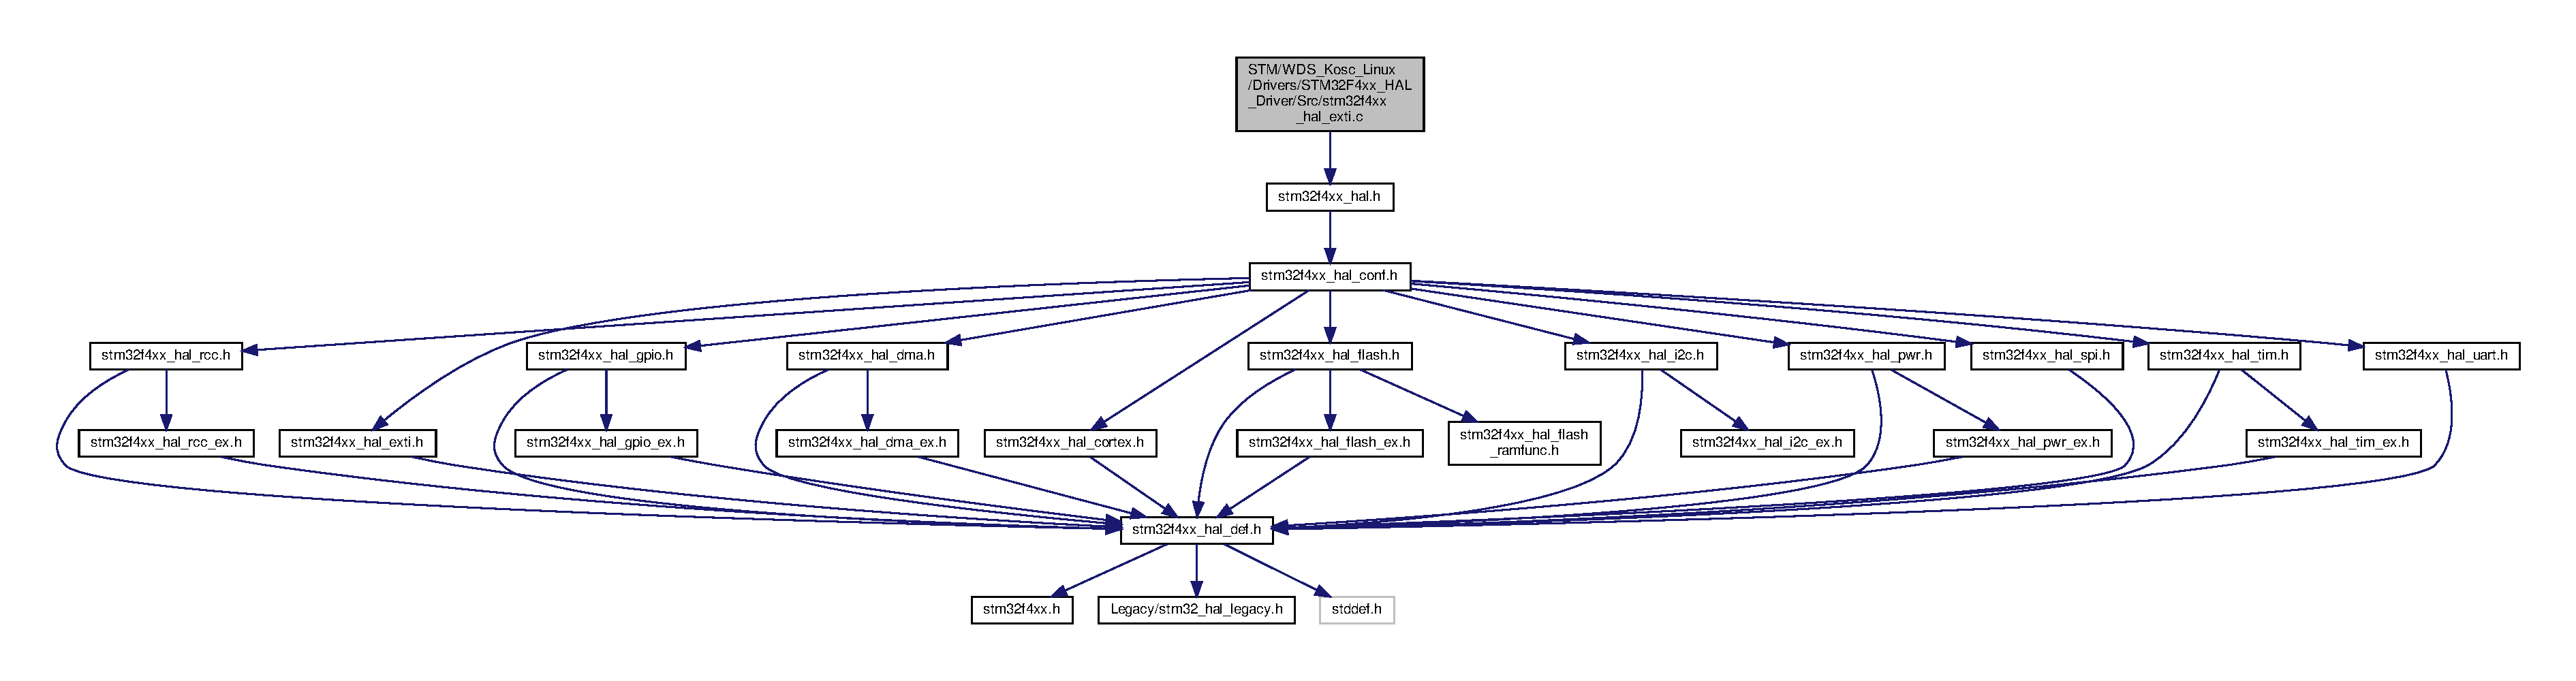
\includegraphics[width=350pt]{stm32f4xx__hal__exti_8c__incl}
\end{center}
\end{figure}


\subsection{Opis szczegółowy}
E\+X\+TI H\+AL module driver. This file provides firmware functions to manage the following functionalities of the Extended Interrupts and events controller (E\+X\+TI) peripheral\+: 

\begin{DoxyAuthor}{Autor}
M\+CD Application Team
\begin{DoxyItemize}
\item Initialization and de-\/initialization functions
\item IO operation functions
\end{DoxyItemize}
\end{DoxyAuthor}
\begin{DoxyVerb}==============================================================================
                  ##### EXTI Peripheral features #####
==============================================================================
[..]
  (+) Each Exti line can be configured within this driver.

  (+) Exti line can be configured in 3 different modes
      (++) Interrupt
      (++) Event
      (++) Both of them

  (+) Configurable Exti lines can be configured with 3 different triggers
      (++) Rising
      (++) Falling
      (++) Both of them

  (+) When set in interrupt mode, configurable Exti lines have two different
      interrupts pending registers which allow to distinguish which transition
      occurs:
      (++) Rising edge pending interrupt
      (++) Falling

  (+) Exti lines 0 to 15 are linked to gpio pin number 0 to 15. Gpio port can
      be selected through multiplexer.

                   ##### How to use this driver #####
==============================================================================
[..]

  (#) Configure the EXTI line using HAL_EXTI_SetConfigLine().
      (++) Choose the interrupt line number by setting "Line" member from
           EXTI_ConfigTypeDef structure.
      (++) Configure the interrupt and/or event mode using "Mode" member from
           EXTI_ConfigTypeDef structure.
      (++) For configurable lines, configure rising and/or falling trigger
           "Trigger" member from EXTI_ConfigTypeDef structure.
      (++) For Exti lines linked to gpio, choose gpio port using "GPIOSel"
           member from GPIO_InitTypeDef structure.

  (#) Get current Exti configuration of a dedicated line using
      HAL_EXTI_GetConfigLine().
      (++) Provide exiting handle as parameter.
      (++) Provide pointer on EXTI_ConfigTypeDef structure as second parameter.

  (#) Clear Exti configuration of a dedicated line using HAL_EXTI_GetConfigLine().
      (++) Provide exiting handle as parameter.

  (#) Register callback to treat Exti interrupts using HAL_EXTI_RegisterCallback().
      (++) Provide exiting handle as first parameter.
      (++) Provide which callback will be registered using one value from
           EXTI_CallbackIDTypeDef.
      (++) Provide callback function pointer.

  (#) Get interrupt pending bit using HAL_EXTI_GetPending().

  (#) Clear interrupt pending bit using HAL_EXTI_GetPending().

  (#) Generate software interrupt using HAL_EXTI_GenerateSWI().\end{DoxyVerb}


\begin{DoxyAttention}{Uwaga}

\end{DoxyAttention}
\subsubsection*{\begin{center}\copyright{} Copyright (c) 2018 S\+T\+Microelectronics. All rights reserved.\end{center} }

This software component is licensed by ST under B\+SD 3-\/\+Clause license, the \char`\"{}\+License\char`\"{}; You may not use this file except in compliance with the License. You may obtain a copy of the License at\+: opensource.\+org/licenses/\+B\+S\+D-\/3-\/\+Clause 